\documentclass{report}
\usepackage{polyglossia}
\usepackage{fixlatvian}
\usepackage{graphicx}
\usepackage{circuitikz}
\usepackage{tabularx}
\usepackage{verbatim}
\usepackage{float}
\usepackage{pgfplots}
\title{Vienkāršu elektrisku shēmu modelēšana}
\author{Viktorija Trofimova}

\begin{document}
\maketitle
% =============================
\chapter{Teorētiskā daļa}

Apēķiniet spriegumus uz rezistoriem 1. attēlā dotajā shēmā. Sprieguma avota V1 spriegu-
ma vērtību U (Voltos) izvēlieties daļskaitli, kas būtu Jūsu apliecības pēdējie trīs cipari dalīti ar
10. Piemēram. ‘ 101REB123 ’ nozīmē V1 = 12.3 (Volti), R1 ir apliecības pēdējo 3 ciparu otrais
numurs+1, R2 ir apliecības numura pēdējais cipars +1. Piemēram, ja Jūsu apliecības numurs
ir ‘ 101REB123 ’ tad ‘ R1=3 ’, ‘ R2=4 ’. Nofotografējiet aprēķinu vai saglabājiet lapiņu. Aprēķina gaita
būs nepieciešama darbā ‘ P02 ’. Turklāt, aprēķins būs jāpievieno atskaitei, ko veiksiet semestra
beigās.

\begin{figure}
\centering
\begin{circuitikz}[scale=1, every node/.style={transform shape}]
\draw
(0,2) to [battery=$V$1] (0,1)
(3,2) to [european resistor=$R1$] (0,2)
(3,2) to [european resistor=$R2$] (3,0)
(3,0) to (0,0)
(0,0) to (0,2);
\end{circuitikz}
\caption{}
\label{fig:sh}
\end{figure}

\begin{figure}[!b]
\centering
\begin{tikzpicture}
\begin{axis}[
    title={$U_{R_{2}}=f(R_2)$},
    xlabel={$R_2$ [$\Omega$]},
    ylabel={$U_{R_{2}}$ [V]},
    xmin=5, xmax=50,
    ymin=5, ymax=15,
    xtick={0,10,20,30,40,50},
    ytick={0,5,10,15},
    ymajorgrids=true,
    xmajorgrids=true,
    grid style=dashed,
]
\addplot[color=blue,]
    coordinates {
    (5,6.71)(10,9.47)(15,11)(20,11.9)(25,12.6)(30,13.1)(35,13.4)(40,13.7)(45,13.9)(50,14.1)
    };
\end{axis}
\end{tikzpicture}
\caption{}
\label{fig:gr}
\end{figure}

\section{Ķēdes aprēķins}
\vspace {1cm}

Tabula \ref{i:tabula} norāda uz ķēdes aprēķiniem, kuri veikti teorētiskajā daļā un tālāk izmantoti  elektrisko shēmu veidošanā, kura redzama \ref{fig:sh} attēlā.

\begin{table}[h]
\centering
\caption{Aprēķini}
\label{i:tabula}
\begin{tabular}[h]{|c|c|}
\hline
R1, R2 & 9 $\Omega$ \\
\hline
V1 & 18.8 $\Omega$ \\
\hline
$U_{R1}$ & 9.4 V \\
\hline
$U_{R2}$ & 9.4 V \\
\hline
\end{tabular}
\end{table}

\chapter{Praktiskā daļa}
\section{Darbs ar GEDA programmām}

\subsection{Darbs ar gschem}
Attēlā \ref{i:gschem} redzama veidotā elektriskā shēma izmantojot gschem.

\begin{figure}[!b]
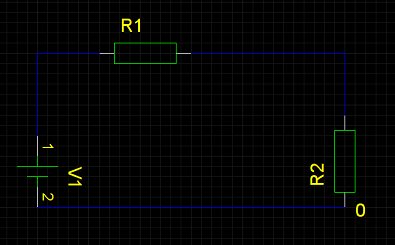
\includegraphics[width=10cm]{atteli/gschem01.png}
\caption{gschem veidotā elektriskā shēma}
\label{i:gschem}
\end{figure}

\subsection{Darbs ar gnetlist}
Zemāk \ref{i:gnetlist} figūrā iespējams redzēt gnetlist darba rezultātus 
\begin{figure}[h!]
\caption{gnetlist}
\label{i:gnetlist}
\begin{verbatim}
* Spice netlister for gnetlist
V1 2 0 18.8
R1 2 1 9
R2 0 1 9
.END
\end{verbatim}
\end{figure}

\subsection{Darbs ar ngspice}
\begin{figure}[t]
\caption{ngspice iegūtie rezultāti}
\label{i:ngspice}
\includegraphics[width=6cm]{atteli/011.ps}
\includegraphics[width=6cm]{atteli/012.ps}
\end{figure}
Attēloti \ref{i:ngspice} ir iegūtie rezultāti, veicot ngspice "plot" attēlu veidošanu un iegūtos rezultātus glabājot ar "hardcopy" funkciju

\section{Darbs ar QUCS programmām}

\subsection{Iegūtās shēmas, tabulas darbā ar QUCS programmu}
\begin{figure}[ht]
\caption{Darbs ar QUCS programmu}
\label{i:qucs}
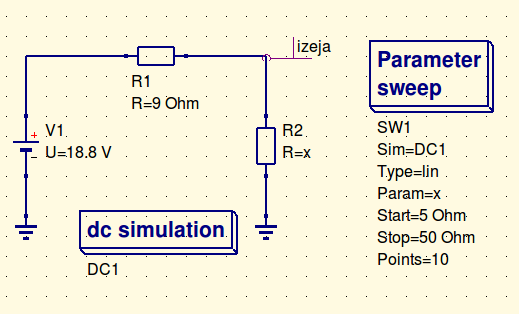
\includegraphics[width=10cm]{atteli/qucs02sch.png}

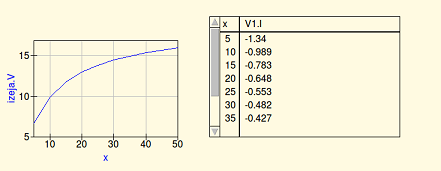
\includegraphics[width=10cm]{atteli/qucskopa.png}
\end{figure}
Iegūtās shēmas un tabulas attēlotas \ref{i:qucs} figurā

\begin{thebibliography}{9}
\bibitem{1} 
\textit{Basic Drawing Using TikZ.} [Skatīts 2018. gada 04. jūnijā].
Pieejams: 
https://www.sharelatex.com/blog/2013/08/27/tikz-series-pt1.html
\bibitem{2} 
\textit{Circuit Diagrams Using Circuitikz.} [Skatīts 2018. gada 04. jūnijā].
Pieejams: 
https://www.sharelatex.com/blog/2013/09/02/tikz-series-pt4.html

 
\end{thebibliography}

\end{document}
% =============================